\section{Background}

\subsection{Program Graph}

Software has been developed with multiple purposes and made 
source code become more complicated. The designing diagram 
is used here to illustrate how source code works. However, 
source code is always changeable to fit with the language 
of developers. Therefore, a program graph is a graph 
that is used to represent the structure of source code and 
to reflect the current version of it.

\begin{figure}[ht!]
    \centering
    \includegraphics[width=0.9\linewidth]{figures/Primitive-Operation-Structure}
    \caption{The Primitive Operations of Structured Programming}
    \label{fig:primitiveoperations}
\end{figure}

\subsubsection{Control Flow Graph}
With difference purposes of software to be developed, 
there are several platforms and languages 
that software developer use for develop software. 
Therefore, it might be difficult for the software tester, 
as he or she may not be familiar with all of these differences. 
CFG is able to represent the structure of source code in 
the form of graph. CFG is Directed Acyclic Graph (DAG) 
that could represent the structure of source code and relationship 
between the lines of code with nodes and edges. It starts from 
the source node to sink node through the sequences of nodes, 
which are connected by edges. CFG with its primitive structure 
was defined by McCabe \cite{McCabe1976}  as shown in 
\figref{fig:primitiveoperations} The software tester should 
analyze CFG and select the test path, which traverses from 
the source node through nodes in the graph with a purpose 
to cover each branch and exercise all predicate nodes in the graph.


\subsubsection{Static Call Graph}
Software is composed of classes, which work together by calling 
their own methods or other methods from other classes. 
SCG, which is a Directed Multiple Graph, represents the relationships 
between classes in SUT, in which each node represents classes 
and edge represents calling of method. In general, there can be 
several outdegree in a single node. SCG is formed by collecting 
calling statements found in source code, in which the called method 
has been called from the calling method for the other classes. 
Only when SCG illustrates the current source code structure, 
the software tester will be able to analyze the interfaces 
between classes to generate a test case that will cover 
all the interfaces in SUT.

\begin{figure}[ht!]
    \centering
    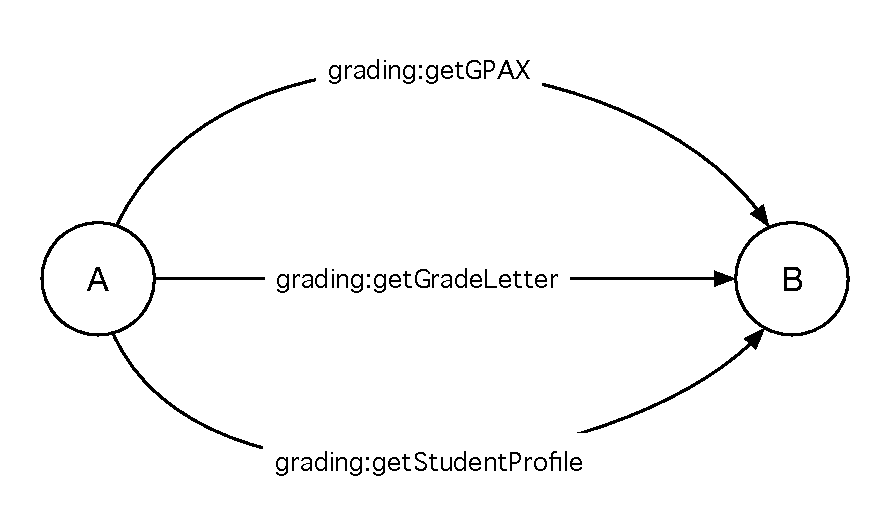
\includegraphics[width=0.9\linewidth]{figures/SCG-A-and-B}
    \caption{Static Call Graph of Class A and Class B}
    \label{fig:scgAandB}
\end{figure}

In \figref{fig:scgAandB} shows an example of SCG that represents 
the relationships between class $A$ and class $B$, Where class $A$ has 
3 calling statements in calling method, grading, that calls 
to called method $getGPAX$, $getGradeLetter$, and $getStudentProfile$ 
in class $B$. Calling and called method are separated with “$:$” 
and used for label the edge between class $A$ and $B$ 
such as “$grading:getGPAX$”. This relationship should be formed into 
$G = (V, E, l, p)$, where $G$ is a Multiple Call Graph, 
$V$ is a set of node, $E$ is a set of edge, $l$ is a set of label, 
$p$ is a function that maps each edge in $E$ to label in $l$. 
For this pair of nodes, $A$ is the head node and $B$ is the tail node 
\cite{Bang-Jensen:2008:DTA:1523254}.
